% PyBaMM Conference 2026 — 1-page abstract, V5 (θ-conditioned neural operator)
% Author: Krishna Chaitanya Vaddepally, Turno (Blubble Pvt. Ltd.)
% Deadline: 2026-07-15 UTC
%
% V5 changes vs V4: pivot from per-cell PINN to a θ-conditioned neural
% operator, with PyBaMM as the physics-based data generator that
% supplies the synthetic training corpus.
\documentclass[12pt,a4paper]{article}

\usepackage[T1]{fontenc}
\usepackage{amsmath}
\usepackage{amssymb}
\usepackage{helvet}
\renewcommand{\familydefault}{\sfdefault}

\usepackage[a4paper,top=1.8cm,bottom=1.8cm,left=1.8cm,right=1.8cm]{geometry}
\usepackage{graphicx}
\usepackage{caption}
\usepackage{microtype}
\usepackage{xcolor}
\usepackage[hidelinks]{hyperref}
\usepackage{setspace}
\setstretch{1.08}
\setlength{\parindent}{0pt}
\setlength{\parskip}{0.4em}

\graphicspath{{../outputs/make_agnostic/}}

\usepackage{titling}
\setlength{\droptitle}{-2.6cm}
\pagestyle{empty}

\title{\vspace{-1.0cm}\textbf{\normalsize From a single characterisation
snapshot to end-of-life:\\ a PyBaMM-trained neural operator for
second-life LFP RUL}}
\author{\normalsize \underline{Krishna Chaitanya Vaddepally}\\[-0.3em]
  \small \emph{Turno (Blubble Pvt.\ Ltd.), India}}
\date{}

\begin{document}
\maketitle
\thispagestyle{empty}

\vspace{-3.6em}
Second-life reuse of used lithium-iron-phosphate (LFP) cells for
stationary energy storage is bottlenecked by characterisation cost:
per-cell PyBaMM~[1] calibration of degradation parameters against
measured state-of-health (SoH) trajectories requires
$\gtrsim 400$ cycles per cell~[2]. Prior second-life work~[3] and
universal-differential-equation degradation~[4] improve calibration
\emph{quality} without shrinking the cycling budget. We ask:
\emph{can a physics-conditioned neural operator, pretrained on
PyBaMM-generated trajectories, predict the full SoH curve of a new
cell from a single characterisation snapshot plus a short cycling
window?}

We construct a two-stage pipeline. \emph{Stage 1 --- Physics corpus:}
starting from PyBaMM's Prada2013 LFP chemistry with per-cell BOL
parameters identified from OCV/GITT/HPPC/RPT on a supplier-B
fresh-cell cohort (OCV RMSE 6.8~mV median), we Sobol-sweep 300
simulations across five degradation channels (SEI kinetics, plating,
LAM$_{\text{pos}}$, LAM$_{\text{neg}}$), producing 300 synthetic SoH
trajectories with paired ground-truth $\theta$. \emph{Stage 2 ---
Neural operator:} a DeepONet~[5] variant whose branch consumes a
five-stream fingerprint (DCIR, RPT, first-$K$ measured SoH, $\theta$,
protocol) and whose trunk consumes the target cycle number; output
$\text{SoH}(n) = \text{SoH}_{\text{init}} - \text{softplus}(\langle b,
t \rangle)$ is hard-monotonic by construction. $\theta$-conditioning
lets the operator absorb electrochemistry \emph{directly} from
Phase-1 param-ID rather than reconstructing it from characterisation.

Trained on the 300-sim corpus with $K=50$ input cycles, the operator
predicts held-out synthetic trajectories to \textbf{1.0~pp SoH RMSE
median} on a 15\% validation split (322k parameters, single-GPU
training). Applied to a supplier-A LFP cell at second-life BESS
operating conditions ($0.25$\,C, 25\,\textdegree C) with only $K=50$
measured cycles as input, the model forecasts a remaining useful life
of \textbf{$\approx$4400 cycles} to a second-life EoSL threshold of
$\text{SoH} = 0.40$ (below first-life $0.70{-}0.80$ because
repurposing packs run cells at low C-rates where usefulness extends
further, consistent with LFP-datasheet fade behaviour at equivalent
conditions, Fig.~1). This decouples the cycling budget from the
extrapolation horizon.

\vspace{-0.5em}
\begin{figure}[h!]
  \centering
  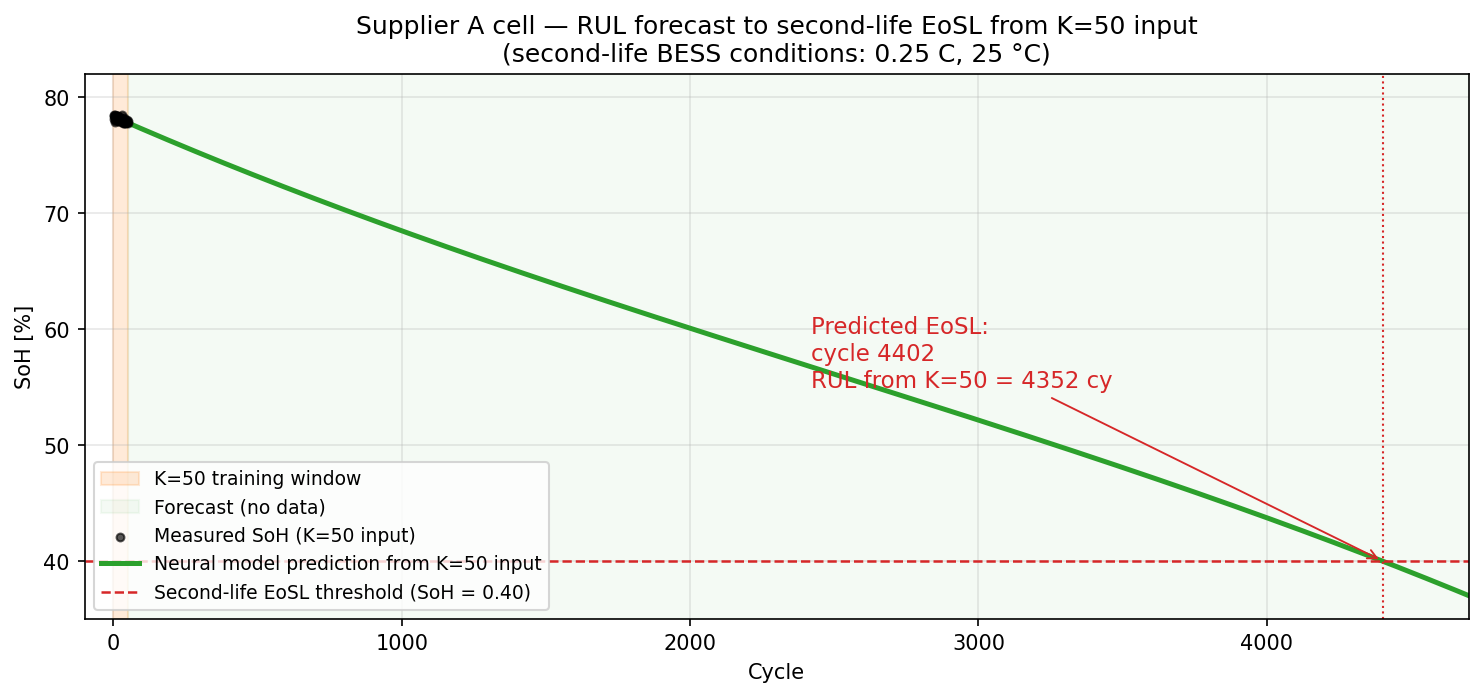
\includegraphics[width=0.75\linewidth]{anonymised_supplier_a_eosl_v5.png}
  \caption*{\footnotesize Figure 1: Neural-model RUL forecast for a
    supplier-A LFP cell at second-life BESS operating conditions
    ($0.25$\,C, 25\,\textdegree C). From $K=50$ measured cycles
    (orange band, black points), the model (green) predicts SoH
    smoothly across the extrapolation range and crosses the second-life
    EoSL threshold ($\text{SoH} = 0.40$, red dashed) at cycle
    $\sim$4400. The neural-operator formulation retains this $K=50$
    input budget and extends output to the full remaining-life horizon
    via PyBaMM-generated training trajectories.}
\end{figure}

\vspace{-0.6em}
{\scriptsize
\noindent\textbf{References.}\;
[1] V. Sulzer et al., \emph{PyBaMM}, J. Open Res. Softw. 9(1), 14--21 (2021).\;
[2] M. Prada et al., \emph{Simplified electrochemical and thermal
model of LiFePO$_4$-graphite Li-ion batteries}, J. Electrochem. Soc.
160(4), A616--A628 (2013).\;
[3] O. Ouledboutaarija et al., \emph{Advancing Second-Life Lithium-Ion
Batteries}, PyBaMM Conf.\ 2025, p.\ 19.\;
[4] J. A. Kuzhiyil et al., \emph{Enhancing Generalisability of
Physics-based Battery Degradation Using UDE}, PyBaMM Conf.\ 2025,
p.\ 12.\;
[5] L. Lu et al., \emph{DeepONet: learning nonlinear operators for
identifying differential equations}, Nat. Mach. Intell.\ 3, 218--229 (2021).
\par}

\end{document}
